%%%%%%%%%%%%%%%%%%%%%%%%%%%%%%%%%%%%%%%
% Wenneker Resume/CV
% LaTeX Template
% Version 1.1 (19/6/2016)
%
% This template has been downloaded from:
% http://www.LaTeXTemplates.com
%
% Original author:
% Frits Wenneker (http://www.howtotex.com) with extensive modifications by 
% Vel (vel@LaTeXTemplates.com)
%
% License:
% CC BY-NC-SA 3.0 (http://creativecommons.org/licenses/by-nc-sa/3.0/
%
%%%%%%%%%%%%%%%%%%%%%%%%%%%%%%%%%%%%%%

% sudo apt install liblatex-driver-perl texlive-fonts-extra texlive-lang-cyrillic

%----------------------------------------------------------------------------------------
%	PACKAGES AND OTHER DOCUMENT CONFIGURATIONS
%----------------------------------------------------------------------------------------

\documentclass[a4paper,12pt]{memoir} % Font and paper size

%%%%%%%%%%%%%%%%%%%%%%%%%%%%%%%%%%%%%%%%%
% Wenneker Resume/CV
% Structure Specification File
% Version 1.1 (19/6/2016)
%
% This file has been downloaded from:
% http://www.LaTeXTemplates.com
%
% Original author:
% Frits Wenneker (http://www.howtotex.com) with extensive modifications by 
% Vel (vel@latextemplates.com)
%
% License:
% CC BY-NC-SA 3.0 (http://creativecommons.org/licenses/by-nc-sa/3.0/)
%
%%%%%%%%%%%%%%%%%%%%%%%%%%%%%%%%%%%%%%%%%

%----------------------------------------------------------------------------------------
%	PACKAGES AND OTHER DOCUMENT CONFIGURATIONS
%----------------------------------------------------------------------------------------

\usepackage{XCharter} % Use the Bitstream Charter font
\usepackage[utf8]{inputenc} % Required for inputting international characters
\usepackage[T1]{fontenc} % Output font encoding for international characters

\usepackage[top=1cm,left=1cm,right=1cm,bottom=1cm]{geometry} % Modify margins

\usepackage{graphicx} % Required for figures

\usepackage{flowfram} % Required for the multi-column layout

\usepackage{url} % URLs

\usepackage[usenames,dvipsnames]{xcolor} % Required for custom colours

\usepackage{tikz} % Required for the horizontal rule

\usepackage{enumitem} % Required for modifying lists
\setlist{noitemsep,nolistsep} % Remove spacing within and around lists

\definecolor{DarkBlue}{rgb}{0,0.2,0.5}

\setlength{\columnsep}{\baselineskip} % Set the spacing between columns

% Define the left frame (sidebar)
\newflowframe{0.2\textwidth}{\textheight}{0pt}{0pt}[left]
\newlength{\LeftMainSep}
\setlength{\LeftMainSep}{0.2\textwidth}
\addtolength{\LeftMainSep}{1\columnsep}

% Small static frame for the vertical line
\newstaticframe{1.5pt}{\textheight}{\LeftMainSep}{0pt}

% Content of the static frame with the vertical line
\begin{staticcontents}{1}
\hfill
\tikz{\draw[loosely dotted,color=DarkBlue,line width=1.5pt,yshift=0](0,0) -- (0,\textheight);}
\hfill\mbox{}
\end{staticcontents}

% Define the right frame (main body)
\addtolength{\LeftMainSep}{1.5pt}
\addtolength{\LeftMainSep}{1\columnsep}
\newflowframe{0.7\textwidth}{\textheight}{\LeftMainSep}{0pt}[main01]

\pagestyle{empty} % Disable all page numbering

\setlength{\parindent}{0pt} % Stop paragraph indentation

%----------------------------------------------------------------------------------------
%	NEW COMMANDS
%----------------------------------------------------------------------------------------

\newcommand{\userinformation}[1]{\renewcommand{\userinformation}{#1}} % Define a new command for the CV user's information that goes into the left column

\newcommand{\cvheading}[1]{{\Huge\bfseries\color{DarkBlue} #1} \par\vspace{.6\baselineskip}} % New command for the CV heading
\newcommand{\cvsubheading}[1]{{\Large\bfseries #1} \vspace{0.2cm}} % New command for the CV subheading

\newcommand{\Sep}{\vspace{1em}} % New command for the spacing between headings
\newcommand{\SmallSep}{\vspace{0.5em}} % New command for the spacing within headings

\newcommand{\aboutme}[2]{ % New command for the about me section
\textbf{\color{DarkBlue} #1}~~#2\par\Sep
}

\newcommand{\CVSection}[1]{ % New command for the headings within sections
{\Large\textbf{#1}}\par
\SmallSep % Used for spacing
}

\newcommand{\CVItem}[2]{ % New command for the item descriptions
\textbf{\color{DarkBlue} #1}\par
#2
\SmallSep % Used for spacing
}

\newcommand{\bluebullet}{\textcolor{DarkBlue}{$\circ$}~~} % New command for the blue bullets
 % Include the file specifying document layout and packages

%----------------------------------------------------------------------------------------
%	NAME AND CONTACT INFORMATION 
%----------------------------------------------------------------------------------------

\userinformation{
\begin{flushright}
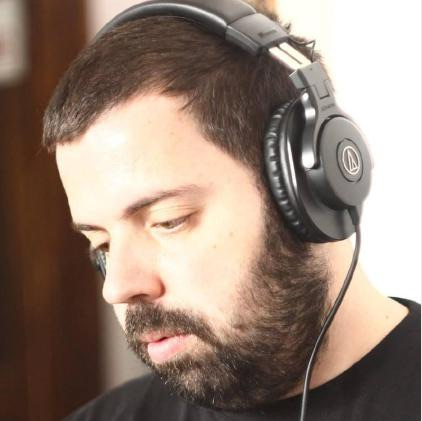
\includegraphics[width=0.6\columnwidth]{photo.jpg}\\[\baselineskip]
\small
\textbf{Filipe Coelho} \\
falktx@falktx.com \\
+49 1573 4020937 \\
+351 969 355 011 \\
\Sep
\textbf{Online Profile} \\
falktx.berlin \\
github.com/falktx \\
patreon.com/falktx \\
social.falktx.berlin \\
\vfill
\end{flushright}
}

%----------------------------------------------------------------------------------------

\begin{document}

\userinformation % Print your information in the left column

\framebreak % End of the first column

%----------------------------------------------------------------------------------------
%	HEADING
%----------------------------------------------------------------------------------------

\cvheading{Filipe Coelho} % Large heading - your name

\cvsubheading{Software Developer} % Subheading - your occupation/specialization

%----------------------------------------------------------------------------------------
%	ABOUT ME
%----------------------------------------------------------------------------------------

\aboutme{About Me}{\\
Self-taught software developer, with personal interest in C++ and Python.\\
Easily motivated by a good challenge. Open-Source enthusiast.
}

%----------------------------------------------------------------------------------------
%	SKILLS
%----------------------------------------------------------------------------------------

\CVSection{Software Development Skills}

%------------------------------------------------

\CVItem{Programming Languages}
{\begin{tabular}{p{0.15\textwidth} p{0.15\textwidth} p{0.15\textwidth} p{0.15\textwidth}}
\bluebullet C & \bluebullet C++ & \bluebullet JavaScript & \bluebullet Python\\
\end{tabular}}

%------------------------------------------------

\CVItem{Programming Frameworks}
{\begin{tabular}{p{0.15\textwidth} p{0.15\textwidth} p{0.15\textwidth} p{0.15\textwidth}}
\bluebullet DPF & \bluebullet JUCE & \bluebullet Qt & \bluebullet HTML5/CSS3/ES6\\
\end{tabular}}

%------------------------------------------------

\CVItem{Programming Systems}
{\begin{tabular}{p{0.3\textwidth} p{0.3\textwidth}}
\bluebullet Bash scripting & \bluebullet Debian packaging\\
\bluebullet Docker & \bluebullet Git\\
\bluebullet POSIX/macOS/win32 APIs & \bluebullet Web Assembly\\
\end{tabular}}

%------------------------------------------------

\CVItem{Created Open-Source Projects}{
\begin{itemize}
	\item \textbf{KXStudio} - \textit{kx.studio} - 2009\\
	  Desktop tools and Debian-based repositories, focused on audio production.\vspace{0.04cm}

	\item \textbf{Cardinal} - \textit{cardinal.kx.studio} - 2021\\
	  Virtual modular synthesizer, based on VCV Rack.\\
	  Self-contained audio plugin and standalone app.\vspace{0.04cm}

	\item \textbf{Carla} - \textit{kx.studio/carla} - 2011\\
	  Fully-featured cross-platform audio plugin host.\\
	  Loads several formats plugins and sample banks, and also works as an audio plugin itself.\vspace{0.04cm}

	\item \textbf{DPF} - \textit{github.com/DISTRHO/DPF} - 2011\\
	  C++ framework to create real-time cross-platform audio plugins.\\
	  Provides UI support using Cairo or OpenGL.\vspace{0.04cm}

	\item \textbf{DPF-Plugins} - \textit{github.com/DISTRHO/DPF-Plugins} - 2012\\
	  A collection of real-time audio plugins, based on DPF.\vspace{0.04cm}

% 	\item \textbf{DISTRHO-Ports} - \textit{distrho.sf.net/ports} - 2011\\
% 	  Linux ports of existing open-source audio plugins, using JUCE.\\
% 	  Contains a forked version of the JUCE library for LV2 plugin support.
\end{itemize}
}

%------------------------------------------------

\Sep % Extra whitespace after the end of a major section

%----------------------------------------------------------------------------------------
%	WORK EXPERIENCE
%----------------------------------------------------------------------------------------

\CVSection{Work Experience}

%------------------------------------------------

\CVItem{September 2015 - September 2017, May 2019 - October 2023, \textit{Lead Software Developer}, MOD Devices GmbH / MOD Audio UG}{
\begin{itemize}
	\item Creation of a highly-optimized, real-time Linux embedded system
	\item Programming of a complex HTML interface and webserver
	\item Programming of real-time audio applications and plugins
\end{itemize}
Technologies used: Buildroot, C, C++, Docker, HTML5, JavaScript, Python
}

%------------------------------------------------

\CVItem{October 2018 - May 2019, \textit{Software Developer}, BEWATEC}{
\begin{itemize}
	\item Full-stack developer
\end{itemize}
Technologies used: AWS, Node Express, Go, ReactJS
}

%------------------------------------------------

\CVItem{September 2017 - October 2018, \textit{Software Developer}, Snuk}{
\begin{itemize}
	\item Full-stack developer
\end{itemize}
Technologies used: Ansible, Django, Docker, Go, GCP, Grafana, ReactJS
}

%------------------------------------------------

% \CVItem{September 2015 - current, \textit{Software Developer}, MOD Duo GbR}{
% \begin{itemize}
% 	\item Creation of a highly-optimized, real-time Linux embedded system
% 	\item Programming of a complex HTML interface and webserver
% 	\item Programming of real-time audio applications and plugins
% \end{itemize}
% Technologies used: Buildroot, C, C++, HTML5, JavaScript, Python
% }

%------------------------------------------------

% \CVItem{April - June 2016, \textit{Software Developer}, Tracktion Software Corp.}{
% \begin{itemize}
% 	\item Programming of real-time audio applications and plugins
% \end{itemize}
% Technologies used: C++, JUCE
% }

%------------------------------------------------

% \CVItem{December 2011 - May 2012, \textit{Software Developer}, TSI}{
% \begin{itemize}
% 	\item Programming of a real-time audio application
% \end{itemize}
% Technologies used: C++, Qt4
% }

%------------------------------------------------

\Sep % Extra whitespace after the end of a major section

%----------------------------------------------------------------------------------------
%	NEW PAGE DELIMITER
%	Place this block wherever you would like the content of your CV to go onto the next page
%----------------------------------------------------------------------------------------

\clearpage % Start a new page

\userinformation % Print your information in the left column

\framebreak % End of the first column

%----------------------------------------------------------------------------------------
%	INTERESTS
%----------------------------------------------------------------------------------------

\CVSection{Interests}

%------------------------------------------------

\CVItem{Professional}{
\begin{itemize}
	\item Creation of desktop applications
	\item Software development focused on high-performance, with real-time requirements in mind
	\item Software with hardware integration
\end{itemize}
}

%------------------------------------------------

\CVItem{Personal}{
\begin{itemize}
	\item Audio production (FL Studio, Renoise and self-made applications)
	\item Linux and Open-Source enthusiast
\end{itemize}
}

%------------------------------------------------

\Sep % Extra whitespace after the end of a major section

%----------------------------------------------------------------------------------------
%	EXTRA ONLINE LINKS
%----------------------------------------------------------------------------------------

\CVSection{Publications and Presentations}

% A small collection of publications about my projects or presentations I did.

%------------------------------------------------

\CVItem{2019, \textit{\small{Past, Present and Future of the JACK Audio Connection Kit}\normalsize}, Sonoj}{
 https://media.ccc.de/v/sonoj2019-1902-jack-past-present-future
\vspace{0.25cm}
}

\CVItem{2018, \textit{\small{An explanation of various plugin formats and why they exist}\normalsize}, Sonoj}{
 https://media.ccc.de/v/sonoj2018-1803-plugin-formats
\vspace{0.25cm}
}

\CVItem{2018, \textit{Carla feature overview and workflows}, Linux Audio Conference}{
 \small
 https://media.ccc.de/v/lac2018-24-carla\_plugin\_host\_feature\_overview\_and\_workflows
 \normalsize
 % \vspace{0.25cm}
}

\CVItem{2017, \textit{Carla Demonstration and Workflows}, Sonoj}{
 https://media.ccc.de/v/sonoj2017-1704-carla-plugin-host
\vspace{0.25cm}
}

\CVItem{2017, \textit{Team presentation about the MOD}, Linux Audio Conference}{
 https://youtu.be/kmil9luagVk
\vspace{0.25cm}
}

\CVItem{2016, \textit{LV2 Plugin Publishing for MOD}, Linux Audio Conference}{
 https://media.ccc.de/v/minilac16-publishingyourlv2
\vspace{0.25cm}
}

\CVItem{2016, \textit{Making Plugins with DPF}, Linux Audio Conference}{
 https://media.ccc.de/v/minilac16-ltsmakesomeplugins
\vspace{0.25cm}
}

\CVItem{2015, \textit{Carla Presentation}, Linux Audio Conference}{
 https://lac.linuxaudio.org/2015/video.php?id=47\&h=576
\vspace{0.25cm}
}

\CVItem{2015, \textit{Testing audio plugins with Carla}, Linux Audio Conference}{
 https://lac.linuxaudio.org/2015/video.php?id=70\&h=576
\vspace{0.25cm}
}

\CVItem{2015, \textit{Personal Interview}, Libre Music Production}{
 https://libremusicproduction.com/articles/friday-interview-2-falktx
\vspace{0.25cm}
}

\CVItem{2015, \textit{Publication about Carla}, Linux Magazine}{
 https://www.linux-magazine.com/Issues/2015/175/Carla
\vspace{0.25cm}
}

\CVItem{2014, \textit{DPF Presentation}, Linux Audio Conference}{
 https://lac.linuxaudio.org/2014/video.php?id=91\&h=720
\vspace{0.25cm}
}

%------------------------------------------------

\Sep % Extra whitespace after the end of a major section

%----------------------------------------------------------------------------------------

\end{document}
